\section{Classifier Design Process}
\label{sec:ClasDes}
As stated in the introduction, a classifier had to be built for two different cases. For both cases, a similar design approach was used. \begin{enumerate}
	\item Investigate the amount of data and use the theory to choose an initial representation method
	\item Train simple classifiers based on the chosen representation method
	\item Perform evaluation
	\item If the performance does not meet the requirements, go back to the theory
	\item If the performance meets the requirements, optimise the system
\end{enumerate}
This approach is visualised in figure \ref{fig:case_design}.
\begin{figure}[H]
	\centering
	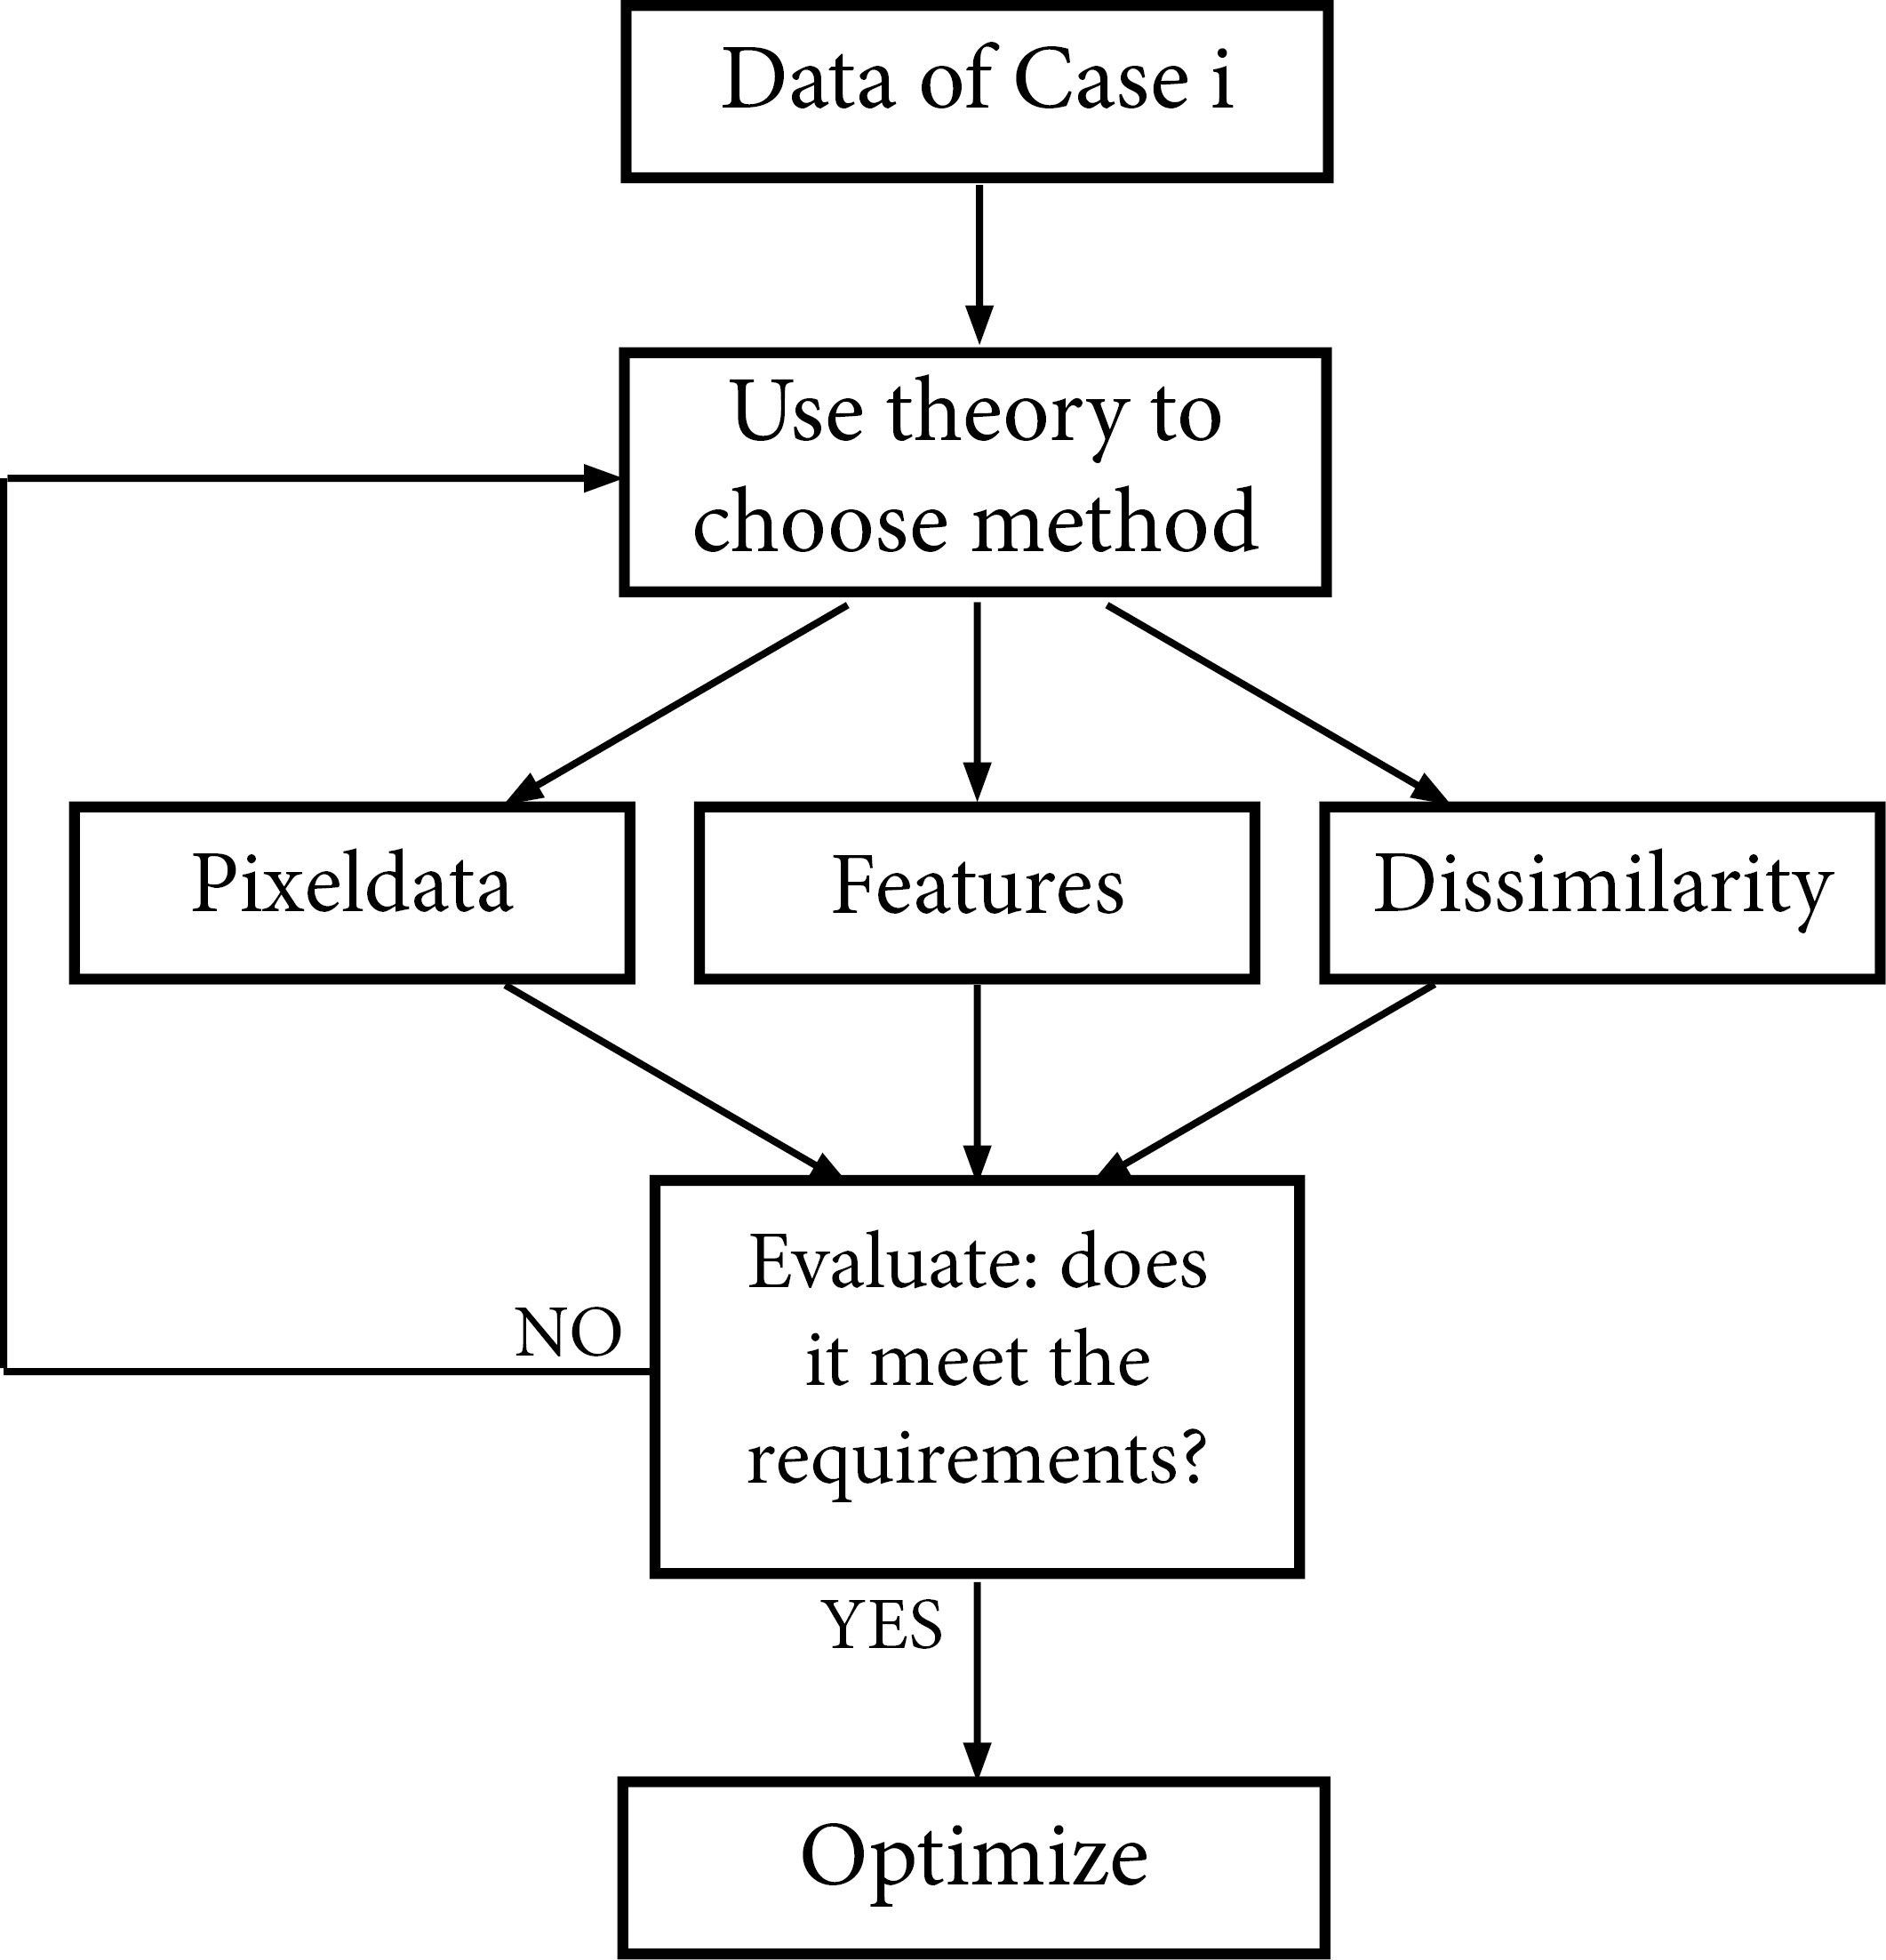
\includegraphics[scale=0.55]{images/Case_Design.jpg}
	\caption{Design-process to determine the best representation method for each of the two cases described in the Introduction.}
	\label{fig:case_design}
\end{figure}
\noindent The image processing described in chapter \ref{sec:ImPros} was kept the same for both cases, with exception of the blob removal in Case 1, because it would take up too much time (see section \ref{sec:Case1} and the recommendations in section \ref{sec:recom} for a more detailed explanation). Furthermore, it is expected that, for the final representation chosen for this case (representation by pixels), the presence of blobs and spots won't influence the performance that much.  The rest of the pre-processing is a very subtle processing and will benefit all potential methods.

\newpage
\section{Case 1}
\label{sec:Case1}
\textbf{Case Summary:} Design a system for training on on the complete dataset, to be applied in the field afterwards.\\
\\
In this scenario the classifying system is trained once, and then applied in the field. This means that all available data can be used as training input, which results in 1000 objects per class, and 10.000 objects in total. (1000 zeros, 1000 ones, etc.) \\
Per representation method, the best classification option will be investigated. For this case, all error rates of the different classifying algorithms were estimated using cross-validation using 10 folds.\\

\subsection{Representation by Pixels}
\subsubsection*{Density Estimating Classifiers}
Large datasets facilitate classification using non-parametric density estimating classifiers. Classifiers of this type are known to perform very well when large datasets are available. After the image preprocessing was carried out as explained in chapter \ref{sec:ImPros}, several density estimating classifiers were tested: Parzen density estimating classifier, which optimizes its ‘width’ parameter iteratively, and k-nearest neighbours classifiers for k = 1,2,3. Although these classifiers are sensitive to uneven scaling of different features, rescaling of feature vectors is not necessary, because all pixel values are within the same range. The results of these classifiers can be seen in table \ref{tab:density}. The images used have a dimension of 16x16 pixels, which results in a 256 dimensional feature-space. The error rates for these classifiers pass the threshold of 5\% already. To investigate the best and worst areas of these classifiers, the error per class was plotted The error per digit class can be observed in figure \ref{fig:errorpdigit}. This shows that errors in ‘8’ and ‘9’ are high for all classifiers, as well as the error for ‘3’, ‘4’ and ‘5’ to a lesser extent. \\
For reference, a quadratic discriminant classifier (QDC) was added to the comparison (see table \ref{tab:density} and figure \ref{fig:errorpdigit}), which is parametric in contrast to the non-parametric classifiers mentioned above. The QDC performs significantly worse than the other classifiers, because it suffers more from the ‘curse of dimensionality’. That is to say that the performance of the classifier benefits from adding more features only up to a certain point, after which the error will rise with extra features added. The ‘curse of dimensionality’ implies that reducing the number of features might decrease the error attained by the classifiers.
\begin{table}[H]
	\centering
	\caption{Overview of the Density-Estimating classifiers and their estimated error.}
	\label{tab:density}
	\begin{tabular}{l|lllll}
		Classifier      & Parzen & 1-NN   & 2-NN   & 3-NN   & QDC    \\ \hline
		Estimated error & 0.0277 & 0.0280 & 0.0343 & 0.0321 & 0.2125
	\end{tabular}
\end{table}
\begin{figure}[H]
	\centering
	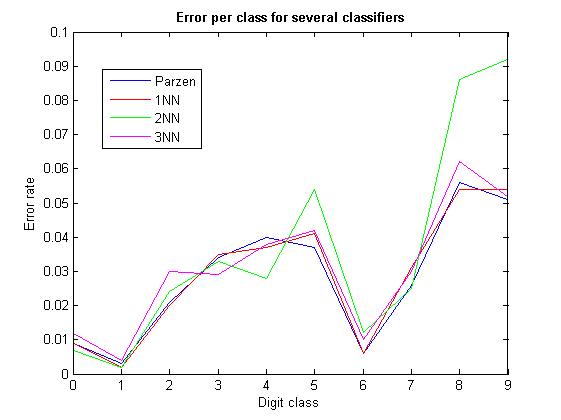
\includegraphics[scale=0.8]{images/pr_figure_2.png}
	\caption{Error per class for different non-parametric density-estimating classifiers.}
	\label{fig:errorpdigit}
\end{figure}
\subsubsection*{Feature Reduction}
Because of the large number of features in the original data set (16x16=256 pixel values) and large number of objects, any feature selection method, especially backwards propagating, will take a significant amount of time. For this reason feature selection methods were discarded, and feature extraction methods were investigated further. \\
The most frequently used feature extraction technique is Principal Component Analysis (PCA). In the PCA-algorithm, it is possible to indicate how much of the total variance should be preserved in the newly created features. The cross-validated error was calculated for the same classifiers as above after applying PCA using values of 0.90 to 0.95 of variance preservation. This range was chosen as it corresponds to the intrinsic dimensionality. Results can be seen in table \ref{tab:PCA}. It is remarkable that the performance of the Parzen classifier deteriorates dramatically, while the performance of the 1-NN classifiers decreases only slightly, and the QD-classifier improves a lot, benefiting from the reduced dimensionality. Note that PCA is an unsupervised method, or in other words: it does not take the class labels or resulting performance of the classifiers into account when choosing new features. This explains the decreased performance of some of the classifiers after using PCA. \\
PCA is sensitive to the scaling of the features. Therefore it is recommended to normalize the variance of the features before applying PCA. In the case of pixel values, however, the data is inherently normalized, because all feature values are in the same range. Applying variance normalization will actually worsen the performance in this case, because it enhances the noise coming from pixels with very low variance. For example: the pixel in the top-left corner will practically always be black, so it has a very low variance. Rescaling will enhance the variance in this pixel, which has unwanted effects. \\
%Addressing the poor performance of the parzen classifier after the application of PCA: even when using PCA to just decrease the dimensionality by 1, from 256 to 255 features, the performance decreases dramatically: from an error of approximately 3\% to an error of 13,57\%.  It is not clear why nearest neighbour algorithms do not seem to suffer from this problem. It might be that the parzen-algorithm suffers from an overlooked effect of PCA. Both the scaling of variance and moving the mean to the origin were empirically ruled out as possible solutions. \\
\\
In figure \ref{fig:errorpdigit2}, the (significantly improved) performance per class for the QD-classifier after applying PCA is compared to the performance as seen in figure \ref{fig:errorpdigit}. It is noteworthy that the values of the QDC curves differ dramatically from the curves for the non-parametric classifiers without dimension reduction. For some classes QDC performs significantly better, while for others the ranking is inverted. This fact can be exploited using classifier combining.
\begin{table}[H]
	\centering
	\caption{Overview of the performance of the classifiers after applying PCA, with different values for the preserved variance.}
	\label{tab:PCA}
	\begin{tabular}{l|llllll}
		Preserved variance       & 0.90   & 0.91   & 0.92   & 0.93   & 0.94   & 0.95   \\
		Resulting dimensionality & 41     & 44     & 48     & 53     & 58     & 65     \\ \hline
		Parzen                   & 0.1122 & 0.1125 & 0.1134 & 0.1136 & 0.1159 & 0.1176 \\
		1-NN                     & 0.0304 & 0.0305 & 0.0314 & 0.0292 & 0.0297 & 0.0297 \\
		QDC                      & 0.0354 & 0.0354 & 0.0375 & 0.0379 & 0.0383 & 0.0361
	\end{tabular}
\end{table}
\begin{figure}[H]
	\centering
	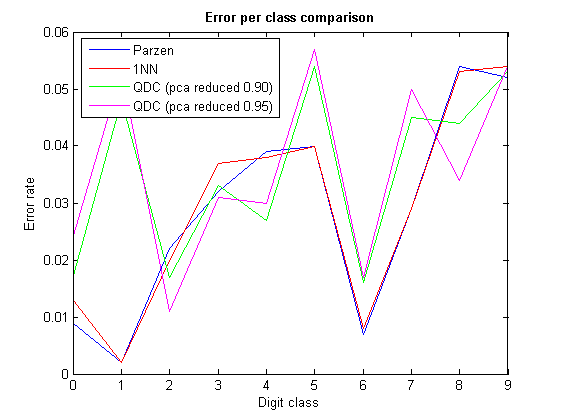
\includegraphics[scale=0.8]{images/pr_figure_3.png}
	\caption{Comparison of the error per class for different classifiers.}
	\label{fig:errorpdigit2}
\end{figure}
\subsubsection*{Combining}
Since the different classifiers in figure \ref{fig:errorpdigit2} perform well for different digit classes, the one alternately performing better than the other, it might be beneficial to combine them. Combining can be carried out using different combining rules. The following combining rules will be investigated: product rule, max rule, mean rule, median rule, min rule. Parzen is to be combined with PCA + QDC, for two different values of variance preservation, as is 1-NN. The result can be seen in table \ref{tab:comb}. The combination using the product rule of Parzen and QDC (after application of PCA preserving 90\% of the variance) offers the best result. The error rate per class can be seen in figure \ref{fig:errorpdigit3}. Except for the digits ‘0’ and ‘1’ (for which Parzen performs best), the combination performs better than the two original classifiers. The ‘9’ is still the digit with the highest classification error.
\begin{table}[H]
	\centering
	\caption{Estimated error for different combinations of classifiers, using different combination rules.}
	\label{tab:comb}
	\begin{tabular}{l|lllll}
		Combining rule                                             & Product & Max    & Mean   & Median & Min    \\ \hline
		\begin{tabular}[c]{@{}l@{}}Parzen\\   + QDC90\end{tabular} & 0.0222  & 0.0271 & 0.0263 & 0.0276 & 0.0333 \\
		\begin{tabular}[c]{@{}l@{}}Parzen\\   + QDC95\end{tabular} & 0.0225  & 0.0274 & 0.0276 & 0.0267 & 0.0367 \\
		\begin{tabular}[c]{@{}l@{}}1-NN\\   + QDC90\end{tabular}   & 0.0361  & 0.0281 & 0.0282 & 0.0285 & 0.0354 \\
		\begin{tabular}[c]{@{}l@{}}1-NN\\   + QDC95\end{tabular}   & 0.0382  & 0.0298 & 0.0281 & 0.0281 & 0.0369
	\end{tabular}
\end{table}
\begin{figure}[H]
	\centering
	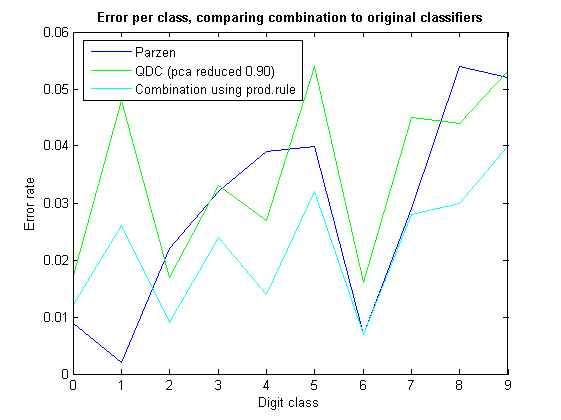
\includegraphics[scale=0.8]{images/pr_figure_4.png}
	\caption{Overview of the error per class of the two original classifiers and their optimal combination.}
	\label{fig:errorpdigit3}
\end{figure}
\subsubsection*{Support Vector Machines}
Support Vector Machines (SVM) are known to be especially useful for classifying in high dimensional feature spaces, which is a major advantage when analysing pixel data. However, the lengthy runtime of the SVM-algorithm is a major disadvantage. Because of the limited time available to analyse the different classifiers, the SVM-algorithm was discarded as a viable option. Once the SVM is created, the runtime of using it to classify and to test it is relatively short. But tweaking and testing it over and over would have taken a significant amount of time. Furthermore, enough training data is available to make adequate density estimations, as is supported by the previous tables and figures.

\subsubsection*{Preliminary Conclusion} for Case 1 with a representation by pixels, the combined classifier (product rule) of Parzen and QDC (using PCA to reduce the dimensionality to 41) gives the best performance, with an error of 0.0222.

\subsection{Representation by Features}
At first glance, the feature representation approach is not the most suitable for scenario 1. Given a large dataset, the performance of the classifiers will benefit from a relatively large number of features. The image analysis methods included in the PRToolbox give 10 features we deemed useful (see Case 2 for a more in-depth discussion of this choice). A number which is predicted to be insufficiently high for achieving an error rate comparable to the rates accomplished using the pixel data approach. Furthermore, because the blob-removal discussed in \ref{sec:ImPros} was not implemented for the large dataset (due to a too large computation time), this method might perform sub-optimal.\\
In order to verify this prediction some indicative tests were carried out, using various classifiers on the dataset containing the extracted features. The tested classifiers are: nearest mean classifier (NMC), Parzen density estimating classifier, 1-nearest neighbour classifier, Linear Discriminant Classifier (LDC), logistic classifier (LOGLC), and quadratic discriminant classifier. In table \ref{tab:feat} the results of these test are shown. For the relevant classifiers (NMC, Parzen, 1-NN) the features were normalized before attempting classification. The resulting error rates are significantly higher than the errors attained above, and have no prospect of improving by feature reduction, because the original dimensionality is low.
\begin{table}[H]
	\centering
	\caption{Overview of the estimated error for different classifiers based on a feature-representation.}
	\label{tab:feat}
	\begin{tabular}{l|llllll}
		Classifier                                                  & NMC    & Parzen & 1-NN   & LDC    & LOGLC  & QDC    \\ \hline
		\begin{tabular}[c]{@{}l@{}}Estimated\\   error\end{tabular} & 0.4454 & 0.3472 & 0.2032 & 0.2178 & 0.1863 & 0.3207
	\end{tabular}
\end{table}
\subsubsection*{Preliminary Conclusion}
The hypothesis is accepted as true, and the feature representation approach is discarded for the large dataset case. The best performing classifier is a Logistic Classifier, with an error of 0.1863. This is not sufficient to surpass the pixel-representation. The feature-representation approach will be dealt with in some more depth in scenario 2, later in this report.

\subsection{Representation by Dissimilarities}
While the main focus for scenario 1 was on the pixel data representation, a brief amount of time was spent on looking at a dissimilarity-representation for the NIST-digits. The dissimilarity-representation offers a better outlook than the feature-representation, because it performs better in higher dimensionalities. In the dissimilarities approach, ‘distances’ to certain ‘prototype’ digits are used as a means of classification. Both the choice of distance measure and the choice of prototype influence the error rate of the resulting classifier. To be able to quickly test the effectiveness of the dissimilarity representation, only the euclidean distance measure was used on case 1. Results are averaged over 3 randomly sampled sets of 10 prototypes per class. The samples remaining in the dataset were used for training (990 samples per class). The results of this quick experiment can be seen in table \ref{tab:diss}. The tested classifiers match those tested for the feature representation.
\begin{table}[H]
	\centering
	\caption{Overview of the estimated error for different classifiers based on a dissimilarity-representation.}
	\label{tab:diss}
	\begin{tabular}{l|llllll}
		Classifier                                                  & NMC    & Parzen & 1-NN   & LDC    & LOGLC  & QDC    \\ \hline
		\begin{tabular}[c]{@{}l@{}}Estimated\\   error\end{tabular} & 0.3487 & 0.0567 & 0.0638 & 0.0741 & 0.0510 & 0.0452
	\end{tabular}
\end{table}
\subsubsection*{Preliminary Conclusion}
The results have improved compared to the feature representation approach, but not exceeded the results of the pixel data approach. PCA was applied to reduce the dimensionality, but this had an adverse effect in this case. The best performing classifier for this representation was a QDC, with an estimated error of 0.0452. \\
To improve results, representative prototypes (a set of very averagely written digits) could be chosen, instead of picked randomly, and alternative dissimilarity measures could be investigated (see the  Discussion in section \ref{sec:DiscConcl}).\\
\subsection{Final Conclusion and Evaluation for Case 1}
As can be seen in table \ref{tab:concase1}, the combination of a Parzen classifier and a QD-classifier applied after PCA, combined using the product rule, yields the best result for scenario 1. 
\begin{table}[H]
	\centering
	\caption{Overview of the best performing classifiers per representation, and their errors.}
	\label{tab:concase1}
	\begin{tabular}{l|ll}
		Representation  & Best Classifier               & Estimated Error \\ \hline
		Pixeldata       & Combination of Parzen and QDC & 0.0222          \\
		Features        & Logistic                      & 0.1863          \\
		Dissimilarities & QDC                           & 0.0452         
	\end{tabular}
\end{table}
\noindent The error of the chosen combined classifier was determined more accurately using cross-validation employing 10 folds, and 10 repetitions. This way some measure of stability can be given, using the standard deviation between the repetitions. The cross-validation yields an error rate of 0.0219 with standard deviation 5.3125e-4. The standard deviation is very small, which means the classifier is stable for different test sets (picked at random from the original dataset).\\
The benchmark test (using \texttt{nist\_eval.m}) yields an error rate of 0.0260 for the chosen classifier for scenario 1. This error is below the desired threshold of 5\%, but is slightly higher than the error found using cross-validation. This might be a result of different class frequencies in the evaluation set compared to the training dataset. In the test set all classes were represented equally often, but in the evaluation set a more realistic class distribution could have been used, increasing the total error rate if this digit has a larger than average misclassification rate. It would not be strange if the frequency of ‘9’ (which has the highest error rate for the used classifier) occurring on bank cheques was slightly higher in practice, due to prices of products often looking like -.99. Note that this last remark is speculation, as there is no way to verify the contents of the evaluation set.





\newpage
\section{Case 2}
\label{sec:Case2}
\textbf{Case Summary:} Design a system for training on each batch of cheques to be processed. The system must be able to correctly classify the handwritten digits after being trained on a maximum of 10 objects per class.\\
\\
\noindent The amount of data available in this case poses some restrictions. While a pixel-data representation worked very well in Case 1, it is likely to have too little data to work with in this case. Some more prior knowledge is needed to handle these batches of cheques. One way of doing this is by letting the system recognize certain distinct properties of the digits. A straight-forward way of doing this is by using a feature representation of the objects. A more abstract way is using a dissimilarity representation.
\\
\subsection{Representation by Features}
To start out, features were chosen as the best representation for this case. The function \texttt{im\_features} from the prtools-toolbox was used to compute 14 different features of all the images in the pre-processed database. Because the amount of features is relatively high compared to the amount of data that is used, some form of feature reduction needs to by applied. MATLABS's forward feature selection (\texttt{featself}) was used initially to get a sense for the features that should be used and the features that could be omitted. This was done for four cases; with and without scaling of the data, and with and without implementing a separate test-set in the \texttt{featself} function. The resulting performance can be seen in figure \ref{fig:featsel_perf}
\begin{figure}[H]
	\centering
	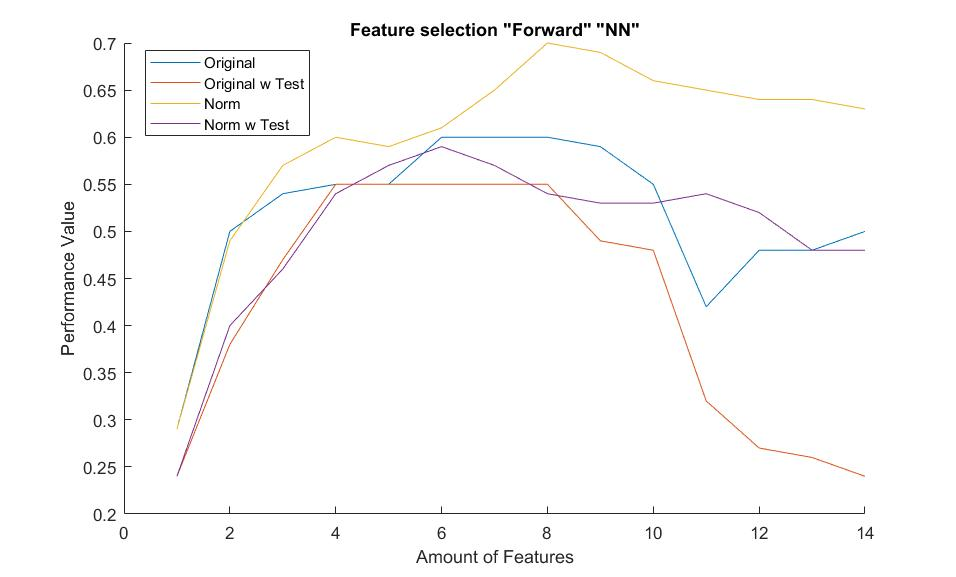
\includegraphics[scale=0.45]{images/featsel_perf.jpg}
	\caption{Performance of features selected by forward feature selection. Both scaling and non-scaling, and with or without test-set are shown.}
	\label{fig:featsel_perf}
\end{figure}
\noindent As can be seen in the figure, there are a lot of differences between the different parameters. There appears to be an optimal amount of features however, somewhere between 4 and 12. In order to get a better grip on which features to use, different feature selection strategies were compared. After the forward selection, the backward and the plus-2-takeaway-1 were tested. This is was done for both the '1-Nearest Neighbor' and the 'Summed Mahalanobis distances' criterion. All these methods indicated that there was an optimum somewhere between 4 and 12 features. However there seemed to be no correlation between which of the features belonged to this optimal set. Therefore a brute force approach was taken. Each possible combination between 3 and 14 features was used for an error-calculation (using the \texttt{testc}  function of PRTools) of four different classifiers (Fischer's Classifier, Linear Classifier, Nearest Mean Classifier and a Nearest Mean Classifier trained on normalized data). After running this setup overnight, the following results were obtained: (see figure \ref{fig:feat_bf_error}).
\begin{figure}[H]
	\centering
	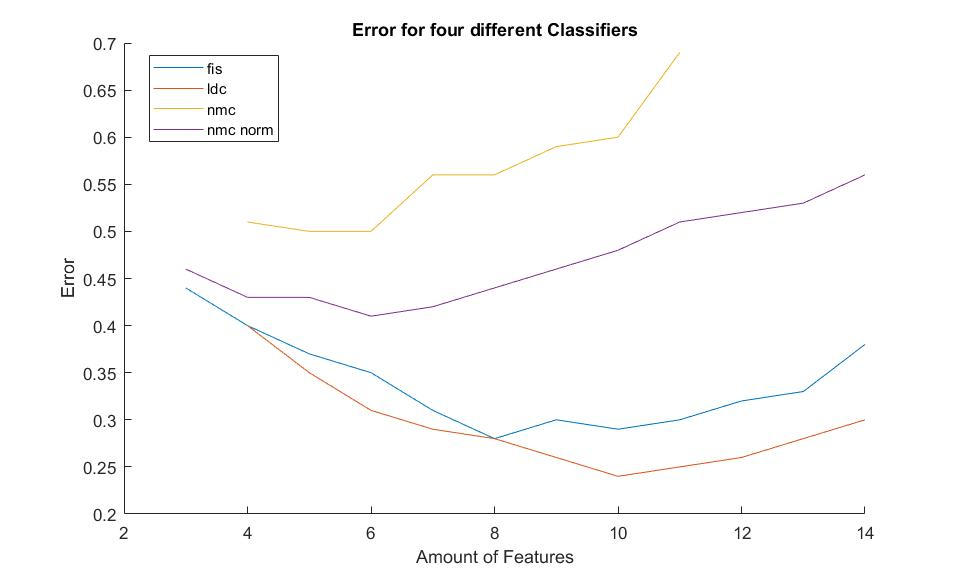
\includegraphics[scale=0.45]{images/feat_bf_error.jpg}
	\caption{Error of different combinations of features for four different trained classifiers; Fischer's (\texttt{fischerc}), Linear Bayes-Normal (\texttt{ldc}), Nearest Mean (\texttt{nmc}) and a normalised version of Nearest Mean.}
	\label{fig:feat_bf_error}
\end{figure}
\noindent This figure shows the lowest error obtained with a certain amount of features. It suggests the optimal amount is 10. It also shows that the Linear Classifier will probably perform best, although even its best error is not under the 25 percent yet. \\
Next, using these 10 features the LDC was trained on different training sets. The result of this was a big fluctuation in errors between datasets, which implies that the set of 10 features were only optimal for one particular dataset. Therefore another brute force approach was used to test all possible combinations of 9 to 12 features on different datasets. In figure \ref{fig:feat_jumps} the error of every combination of 9 features can be seen. Very noticeable are the large drops and jumps in the graph, visualised with the orange line below it. After close inspection of the used features at these points, it was discovered that every increase in error corresponded to the same four features being added, namely 'Convex Area', 'Conves Hull', 'Convex Image' and 'Eccentricity'. A similar pattern was recognized in the other results. It was decided to omit these features, leaving the final dataset with the desired amount of 10 features.
\begin{figure}[H]
	\centering
	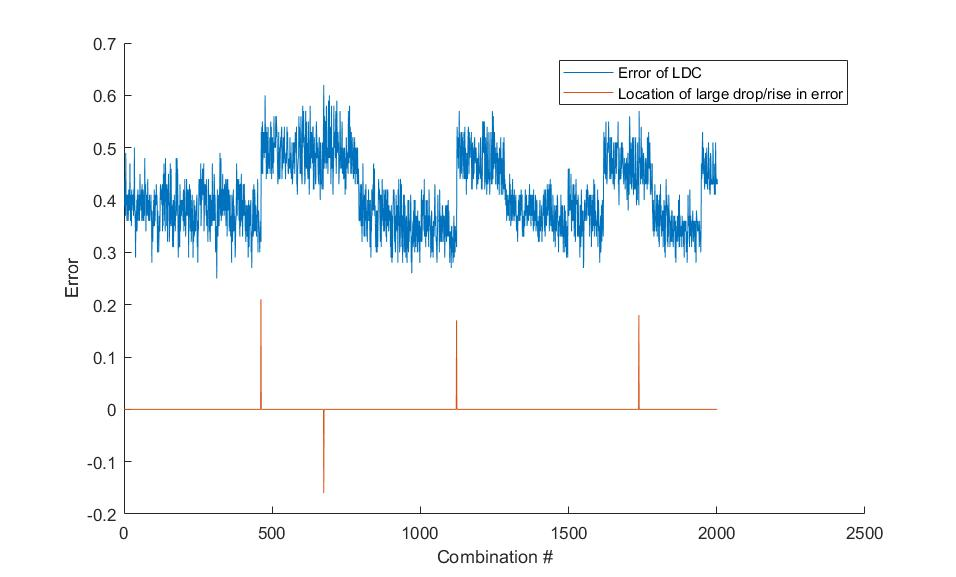
\includegraphics[scale=0.45]{images/feat_jumps.jpg}
	\caption{Error of the LDC-classifier for each possible combination of 10 out of 14 features. The orange line indicates places with a large increase or decrease in error-value.}
	\label{fig:feat_jumps}
\end{figure}

\subsubsection*{Preliminary Conclusion}
\noindent At this time, the complete system consisted of a Linear Classifier (LDC) trained on the dataset from which 10 out of 14 features were selected. Sadly though, test runs of the algorithm yielded an error of 30\%, as can be seen in figure \ref{fig:feat_jumps}. Since this is too high to meet the requirements, a different approach was taken. \\

\subsection{Representation by Dissimilarity}
It was decided that more information needed to be intrinsic in the system in order for it to be able to correctly classify the digits with the small training-set Case 2 provides. Going back to the theory, dissimilarity-representation seemed to be able to do this. By picking a certain amount of representative examples of each digit by hand (the prototypes) and calculating the distance of the remaining objects to these prototypes, correct classification should be possible. \\
\noindent To get an initial idea of the performance of this method, it was first tested whether or not it performed well on the classification of a single class. 90 samples per class were taken, two representative 'ones' were chosen, and the distance between all objects and these two 'ones' was calculated using MATLAB's \texttt{proxm} function. 
\begin{figure}[H]
	\centering
	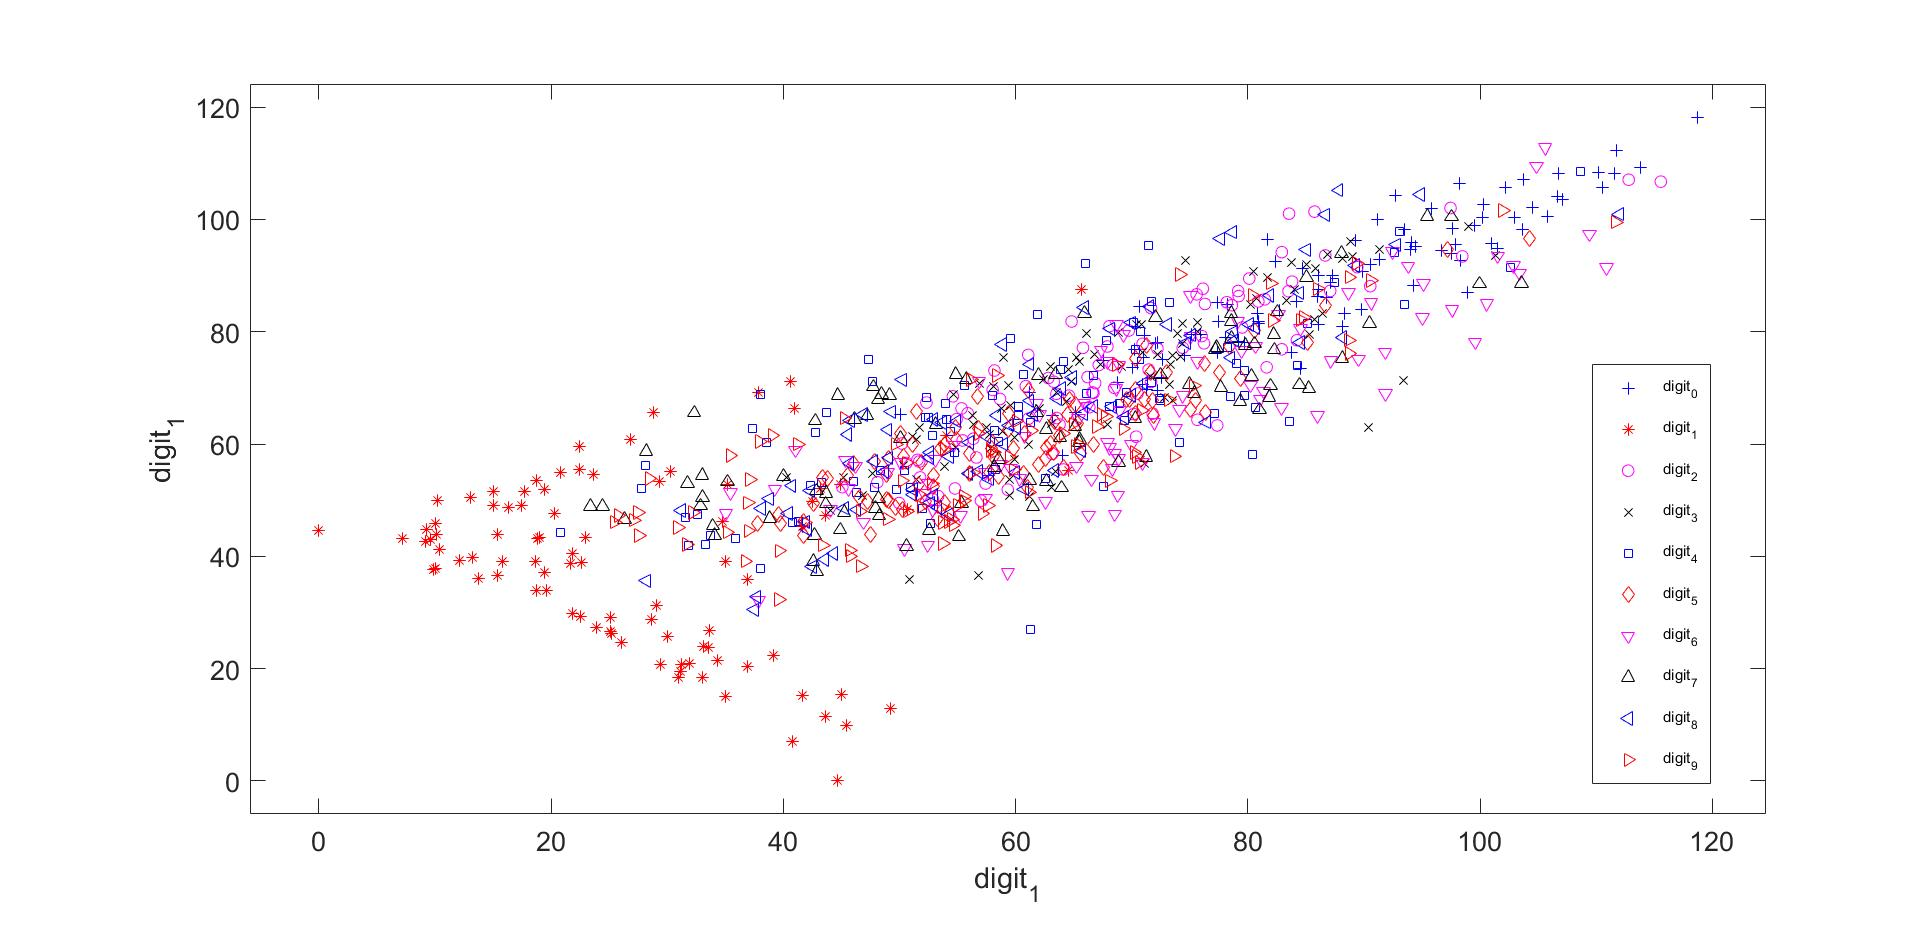
\includegraphics[width = 0.9\textwidth]{images/dissim_two_ones.jpg}
	\caption{Dissimilarity of 90 samples per class to two '1' prototypes, using city-block distances.}
	\label{fig:dissim_two_ones}
\end{figure}
\noindent In figure \ref{fig:dissim_two_ones} a clear clustering of all the 'ones' can be observed. This cluster can be separated from the rest of the objects easily using a linear classifier (for instance LDC).\\
The next step is to get a sense of the optimal distance measure to use with \texttt{proxm}. The estimated error of the LD-classifier was determined for various distance measures. As can be seen in figure \ref{fig:dissim_bar_dist} a few distance measures perform comparable. City-block seemed to be the most consistent over different training sets, so this distance measure was chosen. [1] \\
\begin{figure}[H]
	\centering
	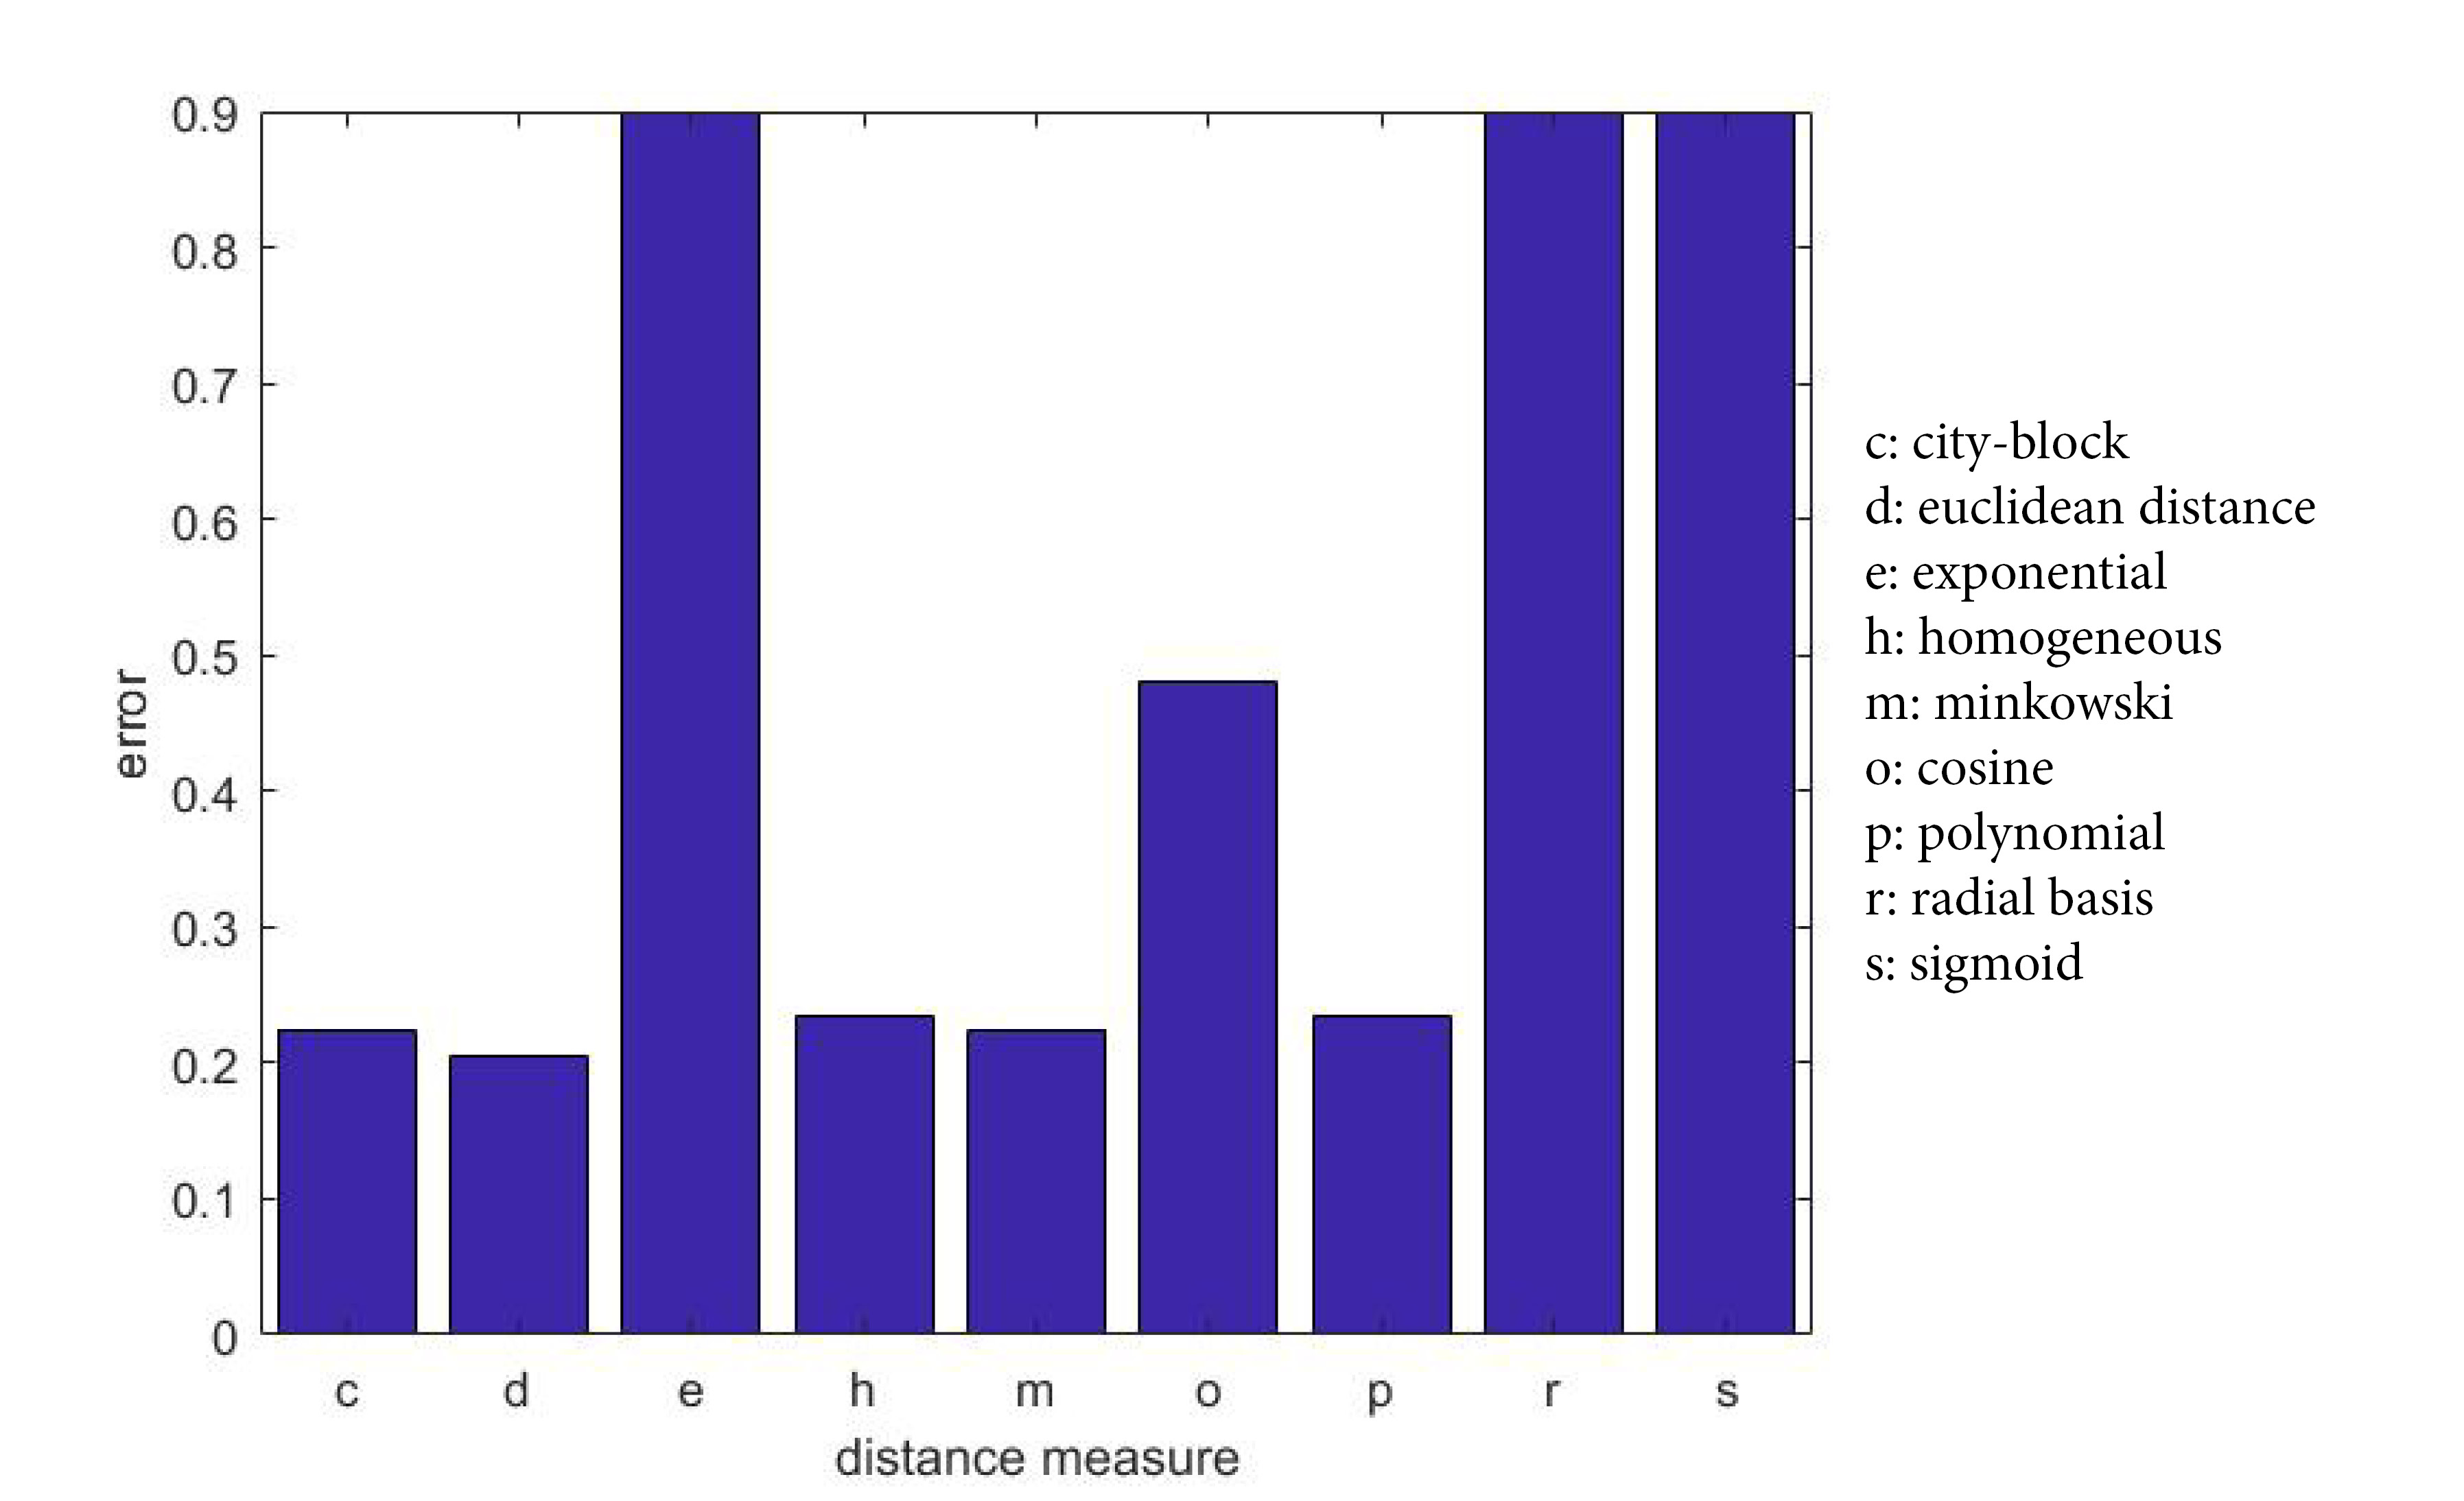
\includegraphics[width = 0.8\textwidth]{images/dissim_bar_dist_legend.jpg}
	\caption{Estimated error of \texttt{LDC} using different distance measures.}
	\label{fig:dissim_bar_dist}
\end{figure}

\noindent This method now has to be scaled up for every class. At the same time, it was realised that manually picking prototypes in Case 2 might not be the best option. This manual selection has to be done for each batch of cheques, through some sort of Graphical User Interface. Because it was assumed that all prototypes should be selected again for each new batch, it was decided to give all objects as prototypes in order to prevent having to code some kind of user interface to manually select prototypes. The resulting high-dimensional feature space would be reduced by means of PCA. Ten samples per class were taken. This resulted in a dataset of 100 samples, each of them having 100 features. Initially, LDC was chosen as the classifier separating the 'ones' from the other digits, but for all classes there might be an other optimal one. Different classifiers were trained after using PCA to reduce the dataset to a wide range of dimmensionalities (dimensionality of 100 means keeping 100 features, so essentially not performing PCA). The results can be seen in table \ref{tab:dissim_all_class} and in figure \ref{fig:dissim_all_class}.
\begin{table}[H]
	\centering
	\caption{Estimated errors for different classifiers, with and without the use of PCA. In the case of PCA, the dimension in which the lowest error is attained is given in the last column.}
	\label{tab:dissim_all_class}
	\begin{tabular}{l|lll}
		Classifier & Without PCA & With PCA & Dimensionality PCA reduces to (lowest error) \\ \hline
		LDC        & 0.243       & 0.2137   & 27                                           \\
		QDC        & 0.9         & 0.4228   & 16                                           \\
		SVC        & 0.2789      & 0.2754   & 80                                           \\
		ParzenC    & 0.2707      & 0.2691   & 32                                           \\
		NMC        & 0.3948      & 0.3947   & 69                                           \\
		kNNC       & 0.3242      & 0.2739   & 54                                          
	\end{tabular}
\end{table}
\begin{figure}[H]
	\centering
	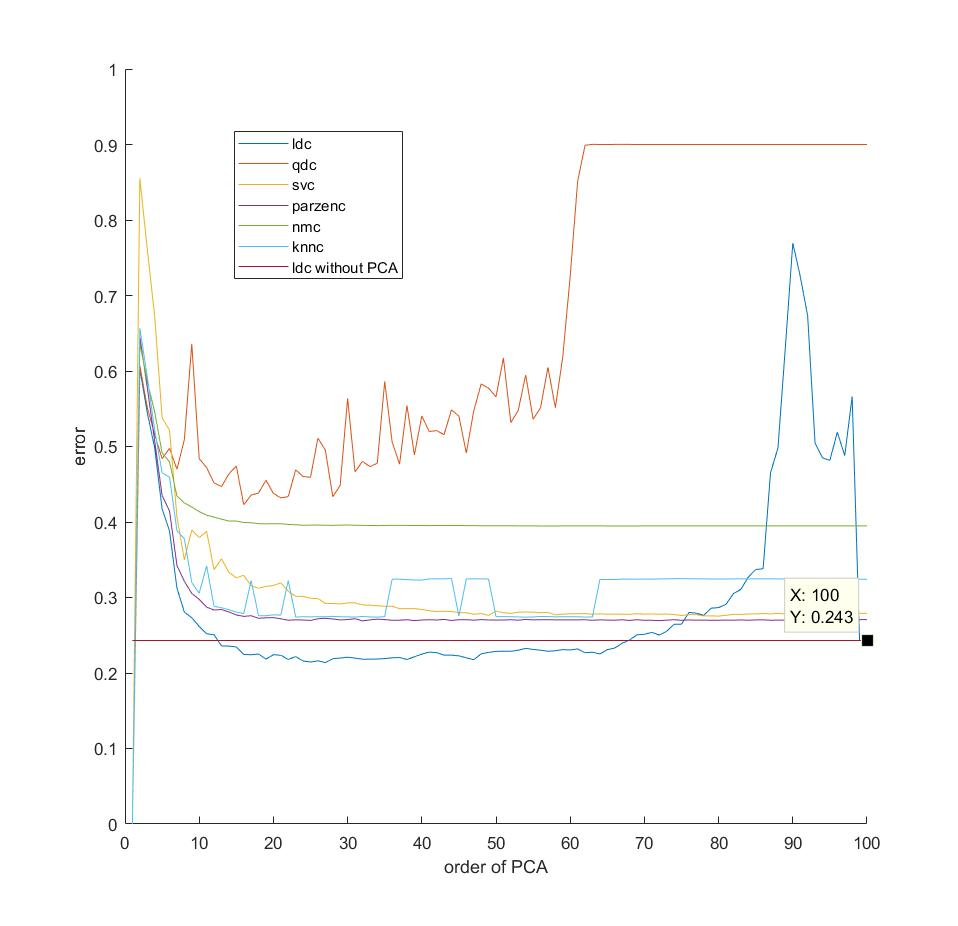
\includegraphics[width = 0.8\textwidth]{images/dissim_all_class.jpg}
	\caption{Estimated error of different classifiers, using PCA resulting in different amounts of dimensions.}
	\label{fig:dissim_all_class}
\end{figure}
\noindent Because of the high dimensionality of the feature space and the relative low amount of samples, the more complex classifiers tend to over-train. This supports the earlier choice of a linear classifier. LDC seems to give the lowest error, both with and without PCA. To find out which one of these performs best, both were trained 10 times on a randomly picked dataset of 10 objects per class, after which they were tested on the remaining 990 objects per class. The results for LDC including all feature reductions (using PCA) and the unaltered LDC are shown in figure \ref{fig:dissim_ldc_mean}.
\begin{figure}[H]
	\centering
	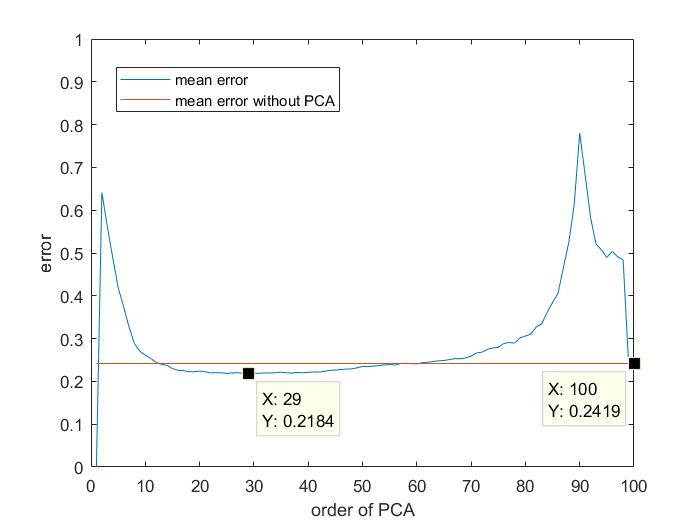
\includegraphics[width = 0.8\textwidth]{images/dissim_ldc_mean.jpg}
	\caption{Average error of ten test stets of \texttt{ldc}.}
	\label{fig:dissim_ldc_mean}
\end{figure}
\subsubsection*{Preliminary Conclusion}
The best performing Classifier using a dissimilarity-representation is a Linear Discriminant Classifier, trained on a dissimilarity-set from which 29 features are extracted using PCA. This classifier has a mean error of 0.2184 with a standard deviation of 0.0153.

\subsection{Representation by Pixels}
Using the pixel representation results in a high dimensionality (16x16=256). The combination of high dimensionality and low training set size suggests that usage of density estimating classifiers can be ruled out in advance. More promising is the use of support vector classifiers, a nearest mean classifier, and perhaps a linear classifier. In table \ref{tab:5er} the estimated error of 5 classifiers is shown. This error was averaged over 10 training sets of 10 objects per class, and tested using a test set containing the other 900 objects of each class. The standard deviation over different training sets is shown in the table as well. The SVC does not perform as well as expected, maybe another kernel would yield a better result.
\begin{table}[H]
	\centering
	\caption{Estimated error of five classifiers for a pixel-representation. The shown error is the average of 10 runs.}
	\label{tab:5er}
	\begin{tabular}{l|lllll}
		Classifier         & NMC    & \begin{tabular}[c]{@{}l@{}}SVC \\ (linear)\end{tabular} & \begin{tabular}[c]{@{}l@{}}SVC \\ (polynomial kernel 2)\end{tabular} & \begin{tabular}[c]{@{}l@{}}SVC \\ (polynomial kernel 3)\end{tabular} & FisherC \\ \hline
		Error              & 0.2676 & 0.3203                                                  & 0.3245                                                               & 0.3303                                                               & 0.5313  \\
		Standard deviation & 0.0182 & 0.0433                                                  & 0.0499                                                               & 0.0325                                                               & 0.0398 
	\end{tabular}
\end{table}
\noindent The huge dimensionality compared to training set size calls for feature reduction. Using PCA preserving 90\% of the variance, the dimensionality was reduced to approximately 20. The results can be seen in table \ref{tab:5erpca}. This decreases the error for the NMC slightly, increases the error for the SVC, and decreases the error for the FisherC dramatically.
\begin{table}[H]
	\centering
	\caption{Estimated error of five classifiers for a pixel-representation, using a PCA to reduce the amount of features. The shown error is the average of 10 runs.}
	\label{tab:5erpca}
	\begin{tabular}{l|lllll}
		Classifier         & NMC    & \begin{tabular}[c]{@{}l@{}}SVC \\ (linear)\end{tabular} & \begin{tabular}[c]{@{}l@{}}SVC \\ (polynomial kernel 2)\end{tabular} & \begin{tabular}[c]{@{}l@{}}SVC\\  (polynomial kernel 3)\end{tabular} & FisherC \\ \hline
		Error              & 0.2631 & 0.3247                                                  & 0.3742                                                               & 0.3661                                                               & 0.2671  \\
		Standard deviation & 0.0179 & 0.0243                                 &  0.0528                                                               & 0.0477                                                               & 0.0181 
	\end{tabular}
\end{table}


\subsubsection*{Preliminary Conclusion}
The best classifier using the pixel representation seems to be the nearest mean classifier, after applying PCA to reduce the dimensionality. The resulting error is approximately 0.2631, with a standard deviation of 0.0179. The classifier is fairly stable over different training sets, but it does not perform well enough to pass the threshold.


\subsection{Final Conclusion and Evaluation for Case 2}
As can be seen in table \ref{tab:concase2}, A Linear Discriminant Classifier with a PCA reducing the feature space to 29 features has the best performance out of all methods that were tried.
\begin{table}[H]
	\centering
	\caption{Overview of the best performing classifiers per representation, and their errors.}
	\label{tab:concase2}
	\begin{tabular}{l|ll}
		Representation  & Best Classifier               & Estimated Error \\ \hline
		Pixeldata       & NMC with PCA &   0.2631        \\
		Features        & LDC with 10 out of 14 selected features                      & $\sim$0.30          \\
		Dissimilarities & LDC with a PCA reducing to 29 features                       &  0.2184        
	\end{tabular}
\end{table}
\noindent The error of the chosen classifier was determined more accurately by training it ten times on 10 samples per class and testing it on the remaining objects. This way some measure of stability can be given, using the standard deviation between the repetitions. This achieved a mean error rate of 0.2184 with standard deviation 0.0153. The standard deviation is quite high, especially compared to Case 1. This is as expected, since the amount of data for Case 2 is limited. (picked at random from the original dataset).\\
The benchmark test (using \texttt{nist\_eval.m}) yields an error rate of 0.194 for the chosen classifier for scenario 2. This error is below the desired threshold of 25\%, and also a bit lower than the estimated error.